\documentclass{pazhb} 

\usepackage[hyperfootnotes=false]{hyperref}

\usepackage{color}
\usepackage{epsf}
\usepackage{amsmath}
\usepackage{amsfonts}
\usepackage{amssymb}
\usepackage{epsf}
\usepackage{graphicx}
\usepackage{gensymb}
\usepackage{float}

\def\procspie{Proc. of the SPIE}
\def\pasj{Publications of the Astronomical Society of Japan}
\def\maxisrc{MAXI\,J1535-571}
\def\maxi{{\em MAXI}}
\def\swiftx{{\em Swift-XRT\,}}
\def\swiftb{{\em Swift-BAT\,}}
\def\xmm{{\em XMM-Newton\,}}
\def\nustar{{\em NuSTAR\,}}
\def\integral{{\em INTEGRAL\,}}
\def\jemx{{\em JEM-X}}
\def\ibis{ {\em IBIS}}


%\newcommand\arcdeg{\mbox{$^\circ$}}
%\newcommand\arcmin{\mbox{$^\prime$}}
%\newcommand\arcsec{\mbox{$^{\prime\prime}$}}%


% \voffset=10mm 
% \hoffset=0mm
% \parindent 8mm
% %######################################################
% \sloppypar


\def\brnote#1{\textcolor{red}{\bf #1}}

\def\ssnote#1{\textcolor{blue}{\bf #1}}


\begin{document}

\journalinfo{2018}{0}{0}{1}[0]
\UDK{524.77}

\title{Эволюция низкочастотных квазипериодических осцилляций в начальной фазе вспышки MAXI J1535-571 }

\author{
  Коллектив ИКИ РАН\email{i.a.mereminskiy@gmail.com}\address{1},
      \addresstext{1}{Институт космических исследований РАН, Москва}
}

\shortauthor{}

\shorttitle{Эволюция НЧ КПО в начальной фазе вспышки MAXI J1535-571}

\submitted{01.12.2017 г.}


\begin{abstract}

  
  \keywords{}

\end{abstract}



%----------------------------------------------------------------------------------------------

\section{Введение}
Третьего сентября 2017 года \cite{negoro17ATel10699} было объявлено об обнаружении телескопом \maxi\, \citep{matsuoka09,negoro16} нового яркого рентгеновского источника, получившего обозначение \maxisrc. Уже через несколько часов, основываясь на данных телескопов {\em XRT} и {\em UVOT} обсерватории {\em Swift}, \cite{kennea17ATel10700} локализовали источник с точностью до 1.5'', что позволило быстро найти оптический компаньон \citep{scaringi17ATel10702}. Источник был также зарегистрирован в радио- \citep{russel17ATel10711} и ближнем-ИК диапазонах \citep{dincer17ATel10716}, а также на миллиметровых волнах \citep{tetarenko17ATel10745}. Дополнительным подтверждением того, что оптический источник действительно является компаньоном рентгеновского, является наличие в ИК-спектре источника линии $Br_{\gamma}$, которую связывают с аккрецией \citep{bandyopadhyay97}. Примерно через неделю после открытия \cite{nakahira17ATel10729} и \cite{kennea17ATel10731} сообщили о начале уменьшения жесткости рентгеновского спектра. 

Подобное поведение является характерным для маломассивных рентгеновских двойных систем с черными дырами. Общепринято описывать ход вспышки в терминах смены ``состояний'', причем каждое состояние имеет свои уникальные спектральные и тайминговые характеристики \citep[подробнее см.][и многие другие]{tanaka96,grebenev97,remillard06,belloni10}. Все подобные вспышки начинаются в низком жестком состоянии, в котором доминирующую роль в излучении играет горячая, оптически тонкая корона. После недолгого роста жесткое состояние сменяется промежуточным-жестким, затем промежуточным-мягким и, наконец, высоким мягким состоянием, в котором большая часть энерговыделения происходит во внутренних частях аккреционного диска. 

Особенный интерес вызывает вопрос о том, на каком расстоянии от компактного объекта происходит разрушение диска во время низкого жесткого состояния и как изменяется это расстояние - называемое радиусом обрезания - в течение вспышки. Результаты имеющихся исследований зачастую противоречивы - в спектрах некоторых систем обнаруживаются холодные аккреционные диски \citep[с температурой в 0.1..0.5 кэВ:][]{miller06, miller06gx339,reis11}, практически достигающие крайней устойчивой орбиты вокруг черной дыры, в то время как ограничения, получающиеся по измерению отраженной компоненты (в частности уширенной линии нейтрального железа на 6.4 кэВ) демонстрируют как большие радиусы обрезания - \cite{furst15_gx339} -, так и малые - \cite{miller15_grs}. 

Как уже было сказано, различные состояния отличаются не только формой спектра, но и характером быстрой переменности \citep{belloni10}. В низком жестком состоянии спектр мощности обычно представляет собой широкополосный шум, на который накладывается один или несколько узких Лоренцианов с частотами от 0.1 до десятков Гц - т.н. низкочастотные квазипериодические осцилляции (НЧ КПО). Известно, что частота слома, выше которой амплитуда широкополосного шума начинает быстро спадать, связана линейным соотношением с фундаментальной частотой КПО \citep{wijnands99}, причем это соотношение выполняется и для систем с черными дырами и с нейтронными звездами, а коэффициент пропорциональности остается единым на протяжении почти трех порядков по частоте. Природа этих НЧ КПО, называемых также КПО типа-C \citep{casella05}, по прежнему неизвестна, однако важно то, что в некоторых моделях происхождения КПО - в моделях релятивистской прецессии \citep{stella98} - частота КПО зависит от радиуса обрезания аккреционного диска. Это предоставляет нам возможность исследовать изменения радиуса обрезания в ходе вспышки, при условии что КПО будет наблюдаться.

Именно такие НЧ КПО были обнаружены нами \citep{mereminskiy17ATel10734} 11 сентября, через восемь дней после открытия \maxisrc и именно им будет посвящена дальнейшая работа.

%----------------------------------------------------------------------------------------------

\section{MAXI J1535-571}
\subsection{Обработка данных}	
Сразу же после обнаружения источника были инициированы интенсивные наблюдательные программы на практически всех работающих в данный момент рентгеновских телескопах. Мы будем использовать данные обсерваторий {\em Swift} (в частности инструментов {\em BAT} \citep{barthelmy05} и {\em XRT} \citep{burrows00})  и \integral\, \citep{winkler03}, а так же данные монитора \maxi и общедоступные наблюдения телескопа \nustar \citep{harrison13_nust}.

В первую очередь нас интересовали данные о переменности источника. Данные телескопа \swiftx\, были пропущены через стандартный конвейер \texttt{xrtpipeline}, затем барицентрированы. Несмотря на то, что фотоприемник \swiftx\, в большей части наблюдений работал в режиме ``перегрузки'' из-за очень большого темпа счета событий, для анализа временной переменности мы не стали прибегать к стандартному приему - исключению столбцов детектора со слишком большим темпом счета - поскольку ``перегрузка'' в первую очередь влияет на измеряемый спектр, и не оказывает существенного влияния на положение центроиды КПО, которое нас интересует. Мы проверили это на нескольких наблюдениях, исключая по пять наиболее засвеченных столбцов детектора. Для анализа использовались кривые блеска с разрешением в 20 мс, в диапазоне 0.8--10 кэВ.

Данные телескопов \jemx\, \citep{lund03} и \ibis\, \citep{ubertini03} обсерватории \integral\, были обработаны стандартным ПО и барицентрированы. Были извлечены кривые блеска с разрешением в 0.05 с в диапазонах 3--20 и 20--200 кэВ, соответственно. К сожалению, в начале 1861 орбиты спутника произошла мощная солнечная вспышка, из-за чего наблюдения были отменены.

Для анализа данных (наблюдение: 90301013002) телескопа \nustar\, был применен стандартный конвейер \texttt{nuproducts}. Для построения кривой блеска в диапазоне 3--78 кэВ использовался круговой регион вокруг источника радиусом в 2', разрешение кривой блеска составило 10 мс. 

\subsection{Профиль вспышки и переход в мягкое состояние}	

Общий профиль вспышки в мягком рентгеновском диапазоне (2--4 и 4--10 кэВ по данным \maxi и в жестком (15--50 кэВ, по данным \swiftb) приведены на Рис.~\ref{fig:lc}. Хорошо видно, что фаза роста вспышки продолжалась в мягком диапазоне вплоть до MJD 58015 (примерно 16 дней), тогда как рост в жестком диапазоне был гораздо более быстрым и занял всего около пяти дней. Как видно из диаграммы интенсивность-жесткость (см. Рис.~\ref{}), переход из жесткого состояния в мягкое произошел около MJD 58015. В этом легко убедиться исходя из спектров мощности, наблюдений \swiftx\, от MJD 58014 и MJD 58017 (ObsID 00010264010 и 00088245002, соответственно). На Рис.~\ref{fig:powtrans} хорошо заметно, что спектр мощности, характерный для жесткого состояния, с ярковыраженным низкочастотным шумом и КПО, сменяется плоским спектром мощности без каких-либо особенностей, характерным для мягкого состояния.
Таким образом, вся фаза роста вспышки заняла примерно 16 дней. Поскольку нас интересуют именно НЧ КПО C-типа, то мы не будем рассматривать дальнейшие данные.

\begin{figure*}
\centerline{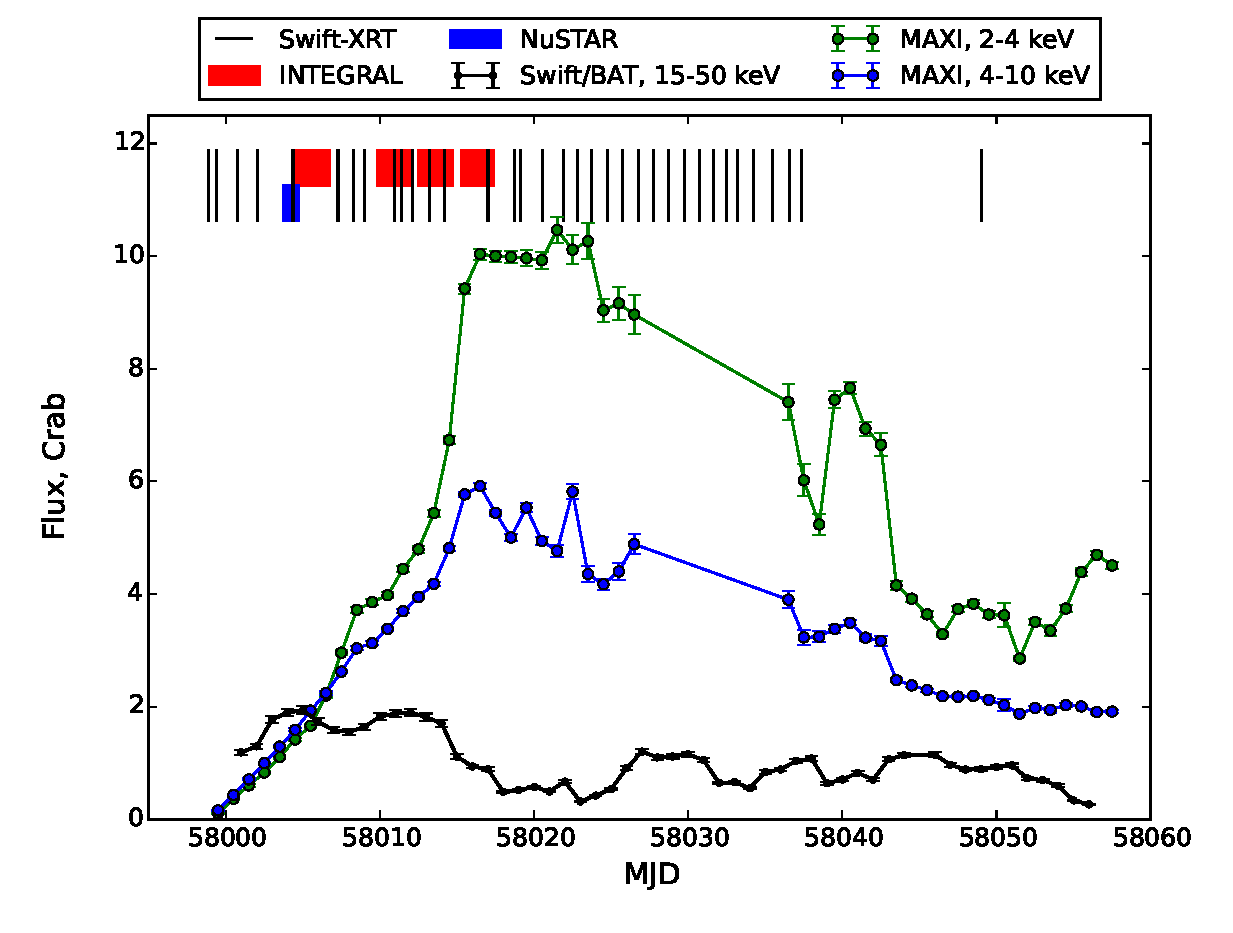
\includegraphics[scale=0.75]{overall_lc_v02.eps}}
\caption{Кривая блеска \maxisrc. Черными точками показан поток в диапазона 15--50 кэВ по данным \swiftb\,, зелеными и синими - данные \maxi\, в диапазонах 2--4 и 4--10 кэВ, соответственно. Красными линиями указаны наблюдения обсерватории \integral\,, черными и синими наблюдения телескопов \swiftx\, и \nustar. }
\label{fig:lc}
\end{figure*} 

\begin{figure}
\centerline{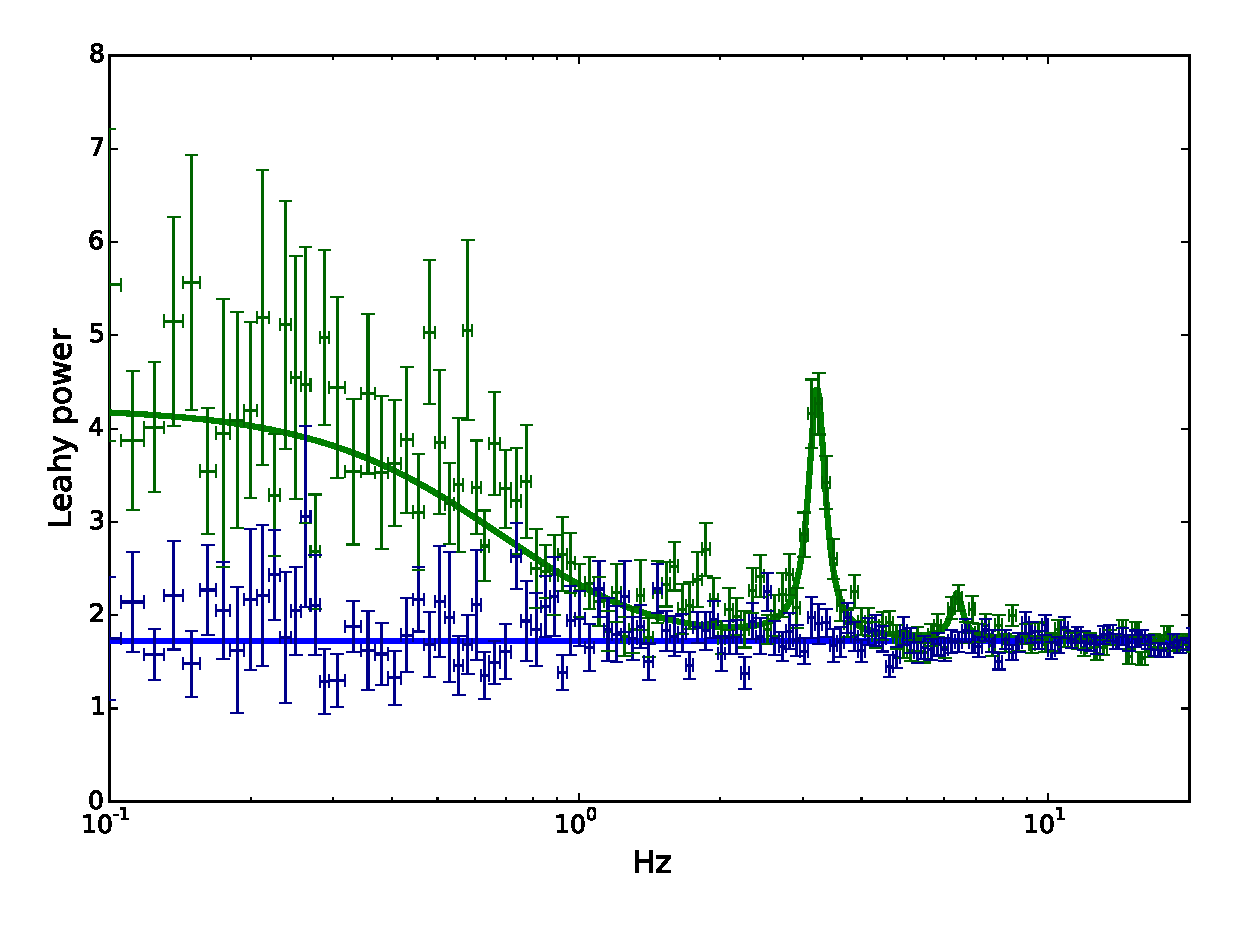
\includegraphics[width=\linewidth]{transition_v01.eps}}
\caption{Спектры мощности \maxisrc\, по данным \swiftx. Зеленые точки и кривая - наблюдение от MJD 58014, до перехода в мягкое состояние, синие - от MJD 58017, после. На спектре мощно до перехода хорошо виден низкочастотный широкополосный шум и два пика КПО, соответствующих фундаментальной частоте и второй гармонике.}
\label{fig:powtrans}
\end{figure}

\begin{table}[t]

\vspace{6mm}
\centering
{{\bf Таблица.} Аппроксимация спектров мощности
источника \mbox{MAXI\,J1535-571},\protect\\}

\vspace{5mm}\begin{tabular}{c|c|c|c} \hline\hline
series & scw start & scw end & QPO frequency\\
$0$ & $02$ & $06$ & $0.23\pm 0.01 $ \\
$1$ & $07$ & $11$ & $0.24\pm 0.01 $ \\
$2$ & $12$ & $16$ & $0.28\pm 0.02 $ \\
$3$ & $17$ & $21$ & $0.37\pm 0.01 $ \\
$4$ & $22$ & $26$ & $0.45\pm 0.01 $ \\
$5$ & $27$ & $31$ & $0.53\pm 0.01 $ \\
$6$ & $32$ & $37$ & $0.68\pm 0.02 $ \\
$7$ & $38$ & $42$ & $0.89\pm 0.02 $ \\
$8$ & $43$ & $47$ & $1.03\pm 0.01 $ \\
\hline
%\multicolumn{6}{l}{}\\ [-3mm]

\end{tabular}
\end{table}





%----------------------------------------------------------------------------------------------


\acknowledgements

\label{lastpage}

%%%%%%%%%%%%%%%%%%%%%%%%%%%%%%%%%%%%%%%%%%%%%%%%%%%%%%%%%%%%%%%%%%%%%%%%%%%%%%%%%%

\bibliographystyle{pazh}
\bibliography{reflist_rus}
\end{document}
